% !TEX root = ms.tex
\documentclass[letterpaper,12pt,oneside]{report}
\pdfoutput=1
% <https://info.arxiv.org/help/submit_tex.html#pdflatex>

% Template info:
% $Date: 2025-09-01 15:40:24 -0400 (Mon, 01 Sep 2025) $
% $Id: ms.tex 2582 2025-09-01 19:40:24Z ben $

\usepackage{lmodern}

% needs to load after fonts
% <https://tex.stackexchange.com/a/586>
\usepackage{microtype}

\usepackage{amsbsy,mathtools,amssymb}

\usepackage[square,numbers]{natbib}
\bibliographystyle{plainnat}

% For double spacing.
% Needs to be loaded before hyperref.
\usepackage{setspace}

\usepackage{hyperref}

% Needed for the `\iflatexml` macro.
\usepackage{latexml}

\usepackage{tikz}
\usetikzlibrary{math}
\usetikzlibrary{decorations.pathmorphing}
\usetikzlibrary{shapes.geometric}
\usetikzlibrary{arrows}

% convenient commands for referencing equations, figures, and tables

\renewcommand*{\eqref}[1]{equation~\ref{eq:#1}}
\newcommand*{\Eqref}[1]{Equation~\ref{eq:#1}}
\newcommand*{\eqsref}[2]{equations~\ref{eq:#1}~and~\ref{eq:#2}}
\newcommand*{\Eqsref}[2]{Equations~\ref{eq:#1}~and~\ref{eq:#2}}
\newcommand*{\eqssref}[3]{equations~\ref{eq:#1},~\ref{eq:#2},~and~\ref{eq:#3}}
\newcommand*{\Eqssref}[3]{Equations~\ref{eq:#1},~\ref{eq:#2},~and~\ref{eq:#3}}
\newcommand*{\eqstoref}[2]{equations~\ref{eq:#1}~to~\ref{eq:#2}}

\newcommand*{\figref}[1]{figure~\ref{fig:#1}}
\newcommand*{\Figref}[1]{Figure~\ref{fig:#1}}
\newcommand*{\figsref}[2]{figures~\ref{fig:#1}~and~\ref{fig:#2}}
\newcommand*{\Figsref}[2]{Figures~\ref{fig:#1}~and~\ref{fig:#2}}
\newcommand*{\figstoref}[2]{figures~\ref{fig:#1}~to~\ref{fig:#2}}
\newcommand*{\Figstoref}[2]{Figures~\ref{fig:#1}~to~\ref{fig:#2}}

\newcommand*{\tabref}[1]{table~\ref{tab:#1}}
\newcommand*{\Tabref}[1]{Table~\ref{tab:#1}}
\newcommand*{\tabsref}[2]{tables~\ref{tab:#1}~and~\ref{tab:#2}}
\newcommand*{\Tabsref}[2]{Tables~\ref{tab:#1}~and~\ref{tab:#2}}

\newcommand*{\secref}[1]{\S~\ref{sec:#1}}
\newcommand*{\Secref}[1]{\S~\ref{sec:#1}}
\newcommand*{\chapref}[1]{chapter~\ref{chap:#1}}
\newcommand*{\Chapref}[1]{Chapter~\ref{chap:#1}}
\newcommand*{\chapsref}[2]{chapters~\ref{chap:#1}~and~\ref{chap:#2}}
%\newcommand*{\chapsecref}[2]{chapter~\ref{chap:#1}, \secref{#2}}
\newcommand*{\Appref}[1]{Appendix~\ref{chap:#1}}
\newcommand*{\appref}[1]{appendix~\ref{chap:#1}}

\newcommand*{\fnref}[1]{footnote~\ref{fn:#1}}
\newcommand*{\fnpageref}[1]{\fnref{#1} on page~\pageref{fn:#1}}

\input{rev.tex}

\author{Ben Trettel}
\title{BlasterSim \gittag\ User's Guide}
\date{\today}

%%%%%%%%%%%%%%%%%%%%%%%%%%%%%%%%%%%%%%%%%%%%%%%%%%%%%%%%%%%%%%%%%%%%%%%%

\begin{document}
\maketitle

\tableofcontents

\chapter{Usage}
\label{usage}

\section{Introduction}
\label{intro}

BlasterSim simulates pneumatic and spring compressed gas guns with a \href{https://en.wikipedia.org/wiki/Lumped-element_model}{lumped parameter} model.

With BlasterSim, you simulate a foam dart blaster or any other compressed gas gun before building.
BlasterSim can also help answer hypothetical questions about an existing build, like whether performance will benefit from a particular change.
Optimal barrel length can be accurately calculated, avoiding inaccurate rules-of-thumb and tedious experiments with varying lengths of barrel.

This guide starts with the usage (\secref{usage}) and theory (\secref{theory}) of BlasterSim.
Later chapters include comparisons of BlasterSim against experimental measurements (\secref{validation}), details of how BlasterSim is tested otherwise (\secref{verification}, how to contribute to BlasterSim (\secref{dev}), and notes on developing BlasterSim (\secref{compiling}).

BlasterSim is under development and not yet feature-complete.

\section{Installation}
\label{installation}

BlasterSim has no dependencies.
BlasterSim is written in Fortran 2018 and will run on any computer a modern Fortran compiler allows.

Obtain the latest BlasterSim binary from \url{http://trettel.us/blastersim/releases/}.
For Linux, this is blastersim-\gittag-linux-x86-64.tgz.
For Windows, this is blastersim-\gittag-windows-x86-64.zip.
For macOS, this is blastersim-\gittag-mac-x86-64.tgz.

The \texttt{blastersim} executable on Linux and macOS and the \texttt{blastersim.exe} executable on Windows can either be placed in the directory you want to run BlasterSim from or placed on your \texttt{PATH}.

See \secref{compiling} for instruction on how to compile BlasterSim from the source tarball or clone of the Git repository.

\section{Running BlasterSim}
\label{running}

With BlasterSim placed in the current directory or your \texttt{PATH}, you can run BlasterSim by typing \texttt{blastersim} in your terminal.

The first command line argument is the input file.
For example, to run BlasterSim on input.nml, type \texttt{blastersim input.nml}.

If BlasterSim is run without an input file (running the command \texttt{blastersim} by itself), BlasterSim will print a message containing information about how to run BlasterSim, the BlasterSim version, and debugging information:
\lstinputlisting[breaklines=true]{blastersim-out.txt}

\section{BlasterSim inputs in general}
\label{inputs-general}

BlasterSim uses Fortran namelist format input files.
Namelist files are broken into groups and variables.
A group starts with the \texttt{\&} symbol, then the name of the group, and contains one or more variables which themselves are the actual input data.
A group ends with the \texttt{/} symbol.
For example, in the example namelist input file below, see that \texttt{group1} group contains the variables \texttt{a}, \texttt{b}, and \texttt{c}.
\texttt{a} is an integer, \texttt{b} is a floating point number (decimal number), and \texttt{c} is a string (which must be quoted).
A namelist file can contain multiple groups.
The example below has two groups, \texttt{group1} and \texttt{group2}.
Comments can be added with the \texttt{!} symbol.
Comments can take up an entire line as in the \texttt{group1} namelist below, or be placed at the end of a line as in the \texttt{group2} namelist below.

\begin{lstlisting}
&group1
a = 0
b = -1.01
c = "string1"
! comment
/

&group2
x = 1
y = 2.05 ! comment
z = "string2"
/
\end{lstlisting}

For more details of the namelist format, refer to the Intel Fortran Compiler documentation~\cite{noauthor_namelist_2025}.

BlasterSim uses SI units in its input files and internally.
Support for other unit systems is not planned due to the complexity of supporting multiple unit systems.
Scientific notation can be used to appropriately scale inputs.
For example, instead of 13 mm being written as \texttt{0.013}, the user can write \texttt{13.0e-3}.

\section{Springer mode}
\label{springer}
% TODO

As shown in \figref{springer time zero}, BlasterSim geometrically models the plunger tube and barrel are treated as cylindrical.
However, BlasterSim does not assume a sudden contraction exists between the plunger tube and barrel as shown by the figure.
That part of the figure is for illustration only.
The connection between the plunger tube and barrel can take any form.

\tikzmath{
\dplunger     = 3;
\lplungertube = 5;
\dbarrel      = 1;
\lbarrel      = 6;
\ldead        = 1.5;
\ylowbarrel   = (\dplunger - \dbarrel)/2; 
\yhighbarrel  = \ylowbarrel + \dbarrel;
\xbarrelend   = \lplungertube + \ldead + \lbarrel;
\xbarrelstart = \lplungertube + \ldead;
\lproj        = 2;
\xproj        = \xbarrelstart + 1;
\xplungerheadstart = 1.5;
\lplungerhead      = 0.5;
\xplungerheadend   = \xplungerheadstart + \lplungerhead;
\ycenter = \dplunger/2;
\yfullspring = -\dplunger/2;
\yfullspringbelow = -7*\dplunger/8;
\yfullspringbelowbelow = -\dplunger;
\yfullspringabove = -\dplunger/4;
\halfyfullspringabove = -1*\dplunger/8;
\lfullspring = 7;
\ylbarrel = \ycenter + (\dplunger + \dbarrel)/4;
\xdead = \lplungertube + \ldead/2;
\xplungerheadunprimed = \lplungertube - \lplungerhead;
\yxz = \ycenter - (\dplunger + \dbarrel)/4;
\xdbarrel  = \xbarrelend - 1;
\xdplunger = \xplungerheadend + 1.0;
}

\begin{figure}
\centering
\begin{tikzpicture}
\draw[thick] (\xbarrelend, \yhighbarrel) -- (\lplungertube, \yhighbarrel) -- (\lplungertube, \dplunger) -- (0, \dplunger) -- (0, 0)         -- (\lplungertube, 0) -- (\lplungertube, \ylowbarrel) -- (\xbarrelend, \ylowbarrel);

\draw[thick,dashed] (\lplungertube, \ylowbarrel) -- (\lplungertube, \yhighbarrel);

\fill[fill=gray,draw=black,thick] (\xproj, \ylowbarrel) rectangle ++(\lproj, \dbarrel);

\fill[fill=gray,draw=black,thick] (\xplungerheadstart, 0) rectangle ++(\lplungerhead, \dplunger);

\tikzstyle{spring}=[thick,decorate,decoration={coil,amplitude=20,segment length=4pt}] % `zigzag` doesn't work right in LaTeXML, but `coil` does
\draw[spring] (0, \ycenter) -- (\xplungerheadstart, \ycenter);

\draw[<->,thick,fill=white] (\xbarrelstart, \ylbarrel) -- node[above] {$l_\text{travel}$} (\xbarrelend, \ylbarrel); % `fill=white` added to make the text fully visible in LaTeXML
\draw[thick,dashed] (\xbarrelend, \yhighbarrel) -- (\xbarrelend, \dplunger);

\node[draw=white] at (\xdead, \ycenter) {$V_\text{dead}$}; % `draw=white` added to make the text fully visible in LaTeXML

\draw[<->,thick] (\xplungerheadend, \halfyfullspringabove) -- node[below] {$y$} (\lplungertube, \halfyfullspringabove);
\draw[thick,dashed] (\lplungertube, \yfullspringabove) -- (\lplungertube, 0);
\draw[thick,dashed] (\xplungerheadend, \yfullspringabove) -- (\xplungerheadend, 0);

\draw[<->,thick] (\lplungertube, \ylbarrel) -- node[above] {$x_\text{0}$} (\xbarrelstart, \ylbarrel);
\draw[thick,dashed] (\xbarrelstart, \ylowbarrel) -- (\xbarrelstart, \dplunger);

\draw[<->,thick] (\lplungertube, \yxz) -- node[below] {$x$} (\xproj, \yxz);
\draw[thick,dashed] (\xproj, 0) -- (\xproj, \ylowbarrel);

\draw[<->,thick] (\xdbarrel, \ylowbarrel) -- node[right] {$d_\text{barrel}$} (\xdbarrel, \yhighbarrel);

\draw[<->,thick] (\xdplunger, \dplunger) -- node[right] {$d_\text{plunger}$} (\xdplunger, 0);
\end{tikzpicture}
\caption{Model spring blaster at arbitrary time as represented in BlasterSim.}
\label{fig:springer time zero}
\end{figure}

\begin{figure}
\centering
\begin{tikzpicture}
\tikzstyle{spring_unprimed}=[thick,decorate,decoration={coil,amplitude=20,segment length=18pt}]
\tikzstyle{spring_full}=[thick,decorate,decoration={coil,amplitude=20,segment length=30pt}]
\draw[thick] (\xbarrelend, \yhighbarrel) -- (\lplungertube, \yhighbarrel) -- (\lplungertube, \dplunger) -- (0, \dplunger) -- (0, 0)         -- (\lplungertube, 0) -- (\lplungertube, \ylowbarrel) -- (\xbarrelend, \ylowbarrel);

\fill[fill=gray,draw=black,thick] (\xplungerheadunprimed, 0) rectangle ++(\lplungerhead, \dplunger);

\draw[spring_unprimed] (0, \ycenter) -- (\xplungerheadunprimed, \ycenter);

\draw[spring_full] (0, \yfullspring) -- (\lfullspring, \yfullspring); % has a long straight line segment in LaTeXML for some reason
\draw[<->,thick] (0, \yfullspringbelow) -- node[below] {$l_\text{spring}$} (\lfullspring, \yfullspringbelow);
\draw[thick,dashed] (0, \yfullspringbelowbelow) -- (0, 0);
\draw[thick,dashed] (\lfullspring, \yfullspringbelowbelow) -- (\lfullspring, 0);

\draw[<->,thick] (\lfullspring, \halfyfullspringabove) -- node[above] {$l_\text{pre}$} (\xplungerheadunprimed, \halfyfullspringabove);
\draw[thick,dashed] (\xplungerheadunprimed, \yfullspringabove) -- (\xplungerheadunprimed, 0);
\end{tikzpicture}
\caption{Unprimed ($y = 0$) model spring blaster as represented in BlasterSim to show spring precompression.}
\label{fig:springer unprimed}
\end{figure}

\begin{figure}
\centering
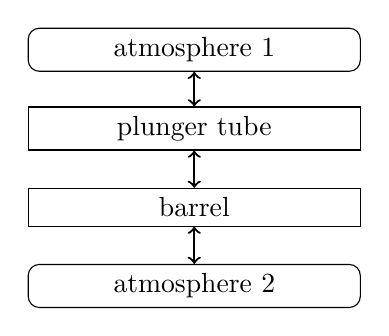
\begin{tikzpicture}
\tikzstyle{cv}       = [rectangle, minimum width=12em, text centered, draw=black]
\tikzstyle{cv_const} = [rectangle, rounded corners, minimum width=12em, text centered, draw=black]
\tikzstyle{arrow}    = [thick, <->]

\node (atm1)         [cv_const]                  {atmosphere~1};
\node (plunger tube) [cv, below of=atm1]         {plunger~tube};
\node (barrel)       [cv, below of=plunger tube] {barrel};
\node (atm2)         [cv_const, below of=barrel] {atmosphere~2};

\draw [arrow] (atm1)         -- (plunger tube);
\draw [arrow] (plunger tube) -- (barrel);
\draw [arrow] (barrel)       -- (atm2);
\end{tikzpicture}
\caption{Abstract connected control volume view of a springer blaster.}
\label{fig:springer control volumes}
\end{figure}

\subsection{\texttt{springer} namelist group variables}
\label{springer-namelist}

The following variables are in the springer namelist group.
If there is a corresponding typeset variable, the notation for that variable is also listed.

\input{geninput_springer.tex}

\subsection{Example springer input file}
\label{springer-example}
% TODO: Go through file and explain what it means.

\lstinputlisting{springer-example.nml}

\section{Pneumatic mode}
\label{pneumatic}
% TODO

\subsection{\texttt{pneumatic} namelist group variables}
\label{pneumatic-namelist}
%TODO

\subsection{Example pneumatic input file}
\label{pneumatic-example}
% TODO: Add example
% TODO: Go through file and explain what it means.

\section{BlasterSim internal model}
\label{internal-model}
% TODO

Internally, BlasterSim simulate blasters using control volumes with arbitrary flow connections between control volumes.
This allows BlasterSim to simulates spring and pneumatic blasters with the same core simulation code. This also allows simulating more atypical blasters without major code changes.

This section describes the internal model in an abstract way.
See \secref{interior-ballistics} for details on the specific equations solved.

\chapter{Theory}\label{theory}

\section{Interior ballistics}\label{interior-ballistics}

\subsection{Control volume variables}
% TODO

% TODO: list all member variables
% TODO: based around control volume mass and energy as presumably this helps with conservation

\subsection{Notation}

% i, j = control volume numbers
% k = gas species
% y = mass fraction

\subsection{Conservation laws}\label{conservation-laws}
% TODO
% mass conservation
% energy conservation

\begin{equation}
    \dv{\dot{m}_{k,i}}{t} = \sum_j \left(y_{k,j} \dot{m}_{j \rightarrow i} - y_{k,i} \dot{m}_{i \rightarrow j}\right)\label{eq:mass conservation}
\end{equation}

\begin{equation}
    \dv{E_i}{t} = -p_i \, A_i \, \dot{x}_i + \sum_j \left(\dot{m}_{j \rightarrow i} h_j - \dot{m}_{i \rightarrow j} h_i\right)\label{eq:energy conservation}
\end{equation}

% TODO: note that definition of $E_i$ could include more than thermal energy and might in the future
\begin{equation}
    E_i = m_i \, u_i
\end{equation}

% TODO: where the pressure work term comes from, why its sign is negative; see moran_fundamentals_2008 p. 39

\subsection{Equations of state}\label{equations-of-state}
% TODO

\begin{equation}
    p_i = \frac{m_i \, R_i \, T_i}{A_i \, x_i}\label{eq:ideal gas eos}
\end{equation}

\subsection{Thermodynamic properties}\label{thermo}
% TODO

% TODO: R from \gamma
% TODO: c_v from R
% TODO: c_p from R
% TODO: mixture u and h

\begin{equation}
    u_{k,i}(T) = u_{0,k} + c_{\text{v},k} \, (T_i - T_{0,k})\label{eq:internal energy}
\end{equation}

\begin{equation}
    h_{k,i}(T) = h_{0,k} + c_{\text{p},k} \, (T_i - T_{0,k})\label{eq:enthalpy}
\end{equation}

\subsection{Connection flow model}\label{connection-flow-model}
% TODO

\citet[ch.~5]{beater_pneumatic_2007}

\subsection{Valve opening model}\label{valve-opening-model}
% TODO

\subsection{Projectile and plunger equations of motion}\label{equations-of-motion}
% TODO

\begin{align}
    \dv{x_i}{t}       &= \dot{x}_i \\
    \dv{\dot{x}_i}{t} &= \frac{A_i}{m_{\text{eff},i}} \left(p_i - p_{\text{mirror},i} - p_{\text{f},i}\right) - \frac{k_i}{m_{\text{eff},i}} \left(x_i + l_{\text{pre},i}\right)
\end{align}

The effective mass of the projectile/plunger factors in the spring mass.
The spring is not moving at a uniform velocity as one end is stationary, so it would be incorrect to add all the spring mass to the effective mass.
The effective mass equation used is
\begin{equation}
    m_{\text{eff},i} = m_{\text{p},i} + C_\text{ms} m_{\text{s},i}\label{eq:effective mass}
\end{equation}
where $C_\text{ms} = \tfrac{1}{3}$ as suggested by \citet{ruby_equivalent_2000} for a stiff spring.

\subsection{Projectile and plunger friction model}\label{friction}
% TODO

\subsection{Plunger impact}\label{plunger-impact}

At the moment, BlasterSim does not handle plunger impact with the end of the plunger tube, and will crash if that occurs.
Plunger impact will be handled in a future version of BlasterSim.

\section{Exterior ballistics}\label{exterior-ballistics}
% TODO

\section{Numerical methods}\label{numerical-methods}

\subsection{Time integration}\label{time-integration}
% TODO

~\cite[p.~1081]{kreyszig_advanced_1993}
~\cite{henon_numerical_1982}

\subsection{Automatic differentiation}\label{autodiff}
% TODO

~\cite{trettel_btrettelflt_2026}

%\subsection{Uncertainty quantification}\label{uncertainty-quantification}
% TODO
% putko_approach_2001

%\subsection{Optimization}\label{optimization}
% TODO
% luke_essentials_2013
% Constraints: deb_efficient_2000 (also discuss modification of this)

% TODO: Also discuss robust optimization
% putko_approach_2001

\chapter{Verification and validation}
\label{verval}

The purpose of this chapter is to help users and potential users of BlasterSim understand how BlasterSim compares against experimental data and also what steps were taken to eliminate bugs in BlasterSim.

BlasterSim has over 200 verification and validation tests at present.
These can be run with \texttt{make check} on Linux and macOS and \texttt{jom check} on Windows.

\section{Verification}
\label{verification}

Verification tests check that the simulation model has been implemented consistently.
In other words, verification tests check that the math of the simulator is consistent with the intended governing equations.
These tests do not test that the governing equations are appropriate in the first place, which is done through BlasterSim's validation tests.

\subsection{Run-time consistency checks}

Every time step, BlasterSim performs internal consistency checks to alert the user if the simulation is becoming inaccurate in a detectable way.
These checks are made in the \texttt{check\_sys} subroutine of cva.f90.
The specific checks performed include:
\begin{itemize}
    \item Whether the simulation ran for too long without the projectile leaving the barrel. (\texttt{run} subroutine return code 1)
    \item Whether a control volume has negative mass. (\texttt{run} subroutine return code 2)
    \item Whether a control volume has negative temperature. (\texttt{run} subroutine return code 3)
    \item Whether the total system mass deviates from the starting mass by more than 0.001\%. (\texttt{run} subroutine return code 4)
    \item Whether the total system energy deviates from the starting energy by more than 0.01\%. (\texttt{run} subroutine return code 5)
    \item If automatic differentiation is used, whether any component of the gradient of the total system mass deviates by more than a set amount. (\texttt{run} subroutine return code 6)
    \item If automatic differentiation is used, whether any component of the gradient of the total system energy deviates by more than a set amount. (\texttt{run} subroutine return code 7)
    \item Whether the ideal gas equation of state has become inaccurate due to the pressure increasing above the critical pressure. (\texttt{run} subroutine return code 8)
    \item Whether the coordinates of any piston become desynchronized between control volumes on either side of the mentioned piston. (\texttt{run} subroutine return code 9)
\end{itemize}

\subsection{Debugging run-time assertions}

BlasterSim contains hundreds of run-time assertions which perform deeper internal consistency checks.
These additional checks are disabled in the released versions of BlasterSim for speed but are enabled during all developer testing runs for debugging purposes.

\subsection{Comparison with exact solution}

To test that the time integration in BlasterSim is working correctly, an exact solution for a simple case was constructed.
This case has only two control volumes, one for the barrel, and one for the atmosphere.
See \figref{exact solution} for an illustration of this test case.

\tikzmath{
\dtube     = 1;
\ltube     = 12;
\lproj     = 2;
\xproj     = 3;
\lx        = -\dtube/2;
\yxdash    = -\dtube;
\ytubedash = 2*\dtube;
\yxcvtext  = \dtube/2;
\xbarreltext = \xproj/2;
\xatmtext    = \xproj + \lproj + 3;
}

\begin{figure}
\centering
\begin{tikzpicture}
\draw[thick] (\ltube, \dtube) -- (0, \dtube) -- (0, 0) -- (\ltube, 0);

\fill[fill=gray,draw=black,thick] (\xproj, 0) rectangle ++(\lproj, \dtube);

\draw[<->,thick]    (0, \lx)    -- node[below] {$x$} (\xproj, \lx);
\draw[thick,dashed] (0, 0)      -- (0, \yxdash);
\draw[thick,dashed] (\xproj, 0) -- (\xproj, \yxdash);

% `draw=white` added to make the text fully visible in LaTeXML
\node[draw=white] at (\xbarreltext, \yxcvtext) {barrel};
\node[draw=white] at (\xatmtext,    \yxcvtext) {atmosphere};
\end{tikzpicture}
\caption{Test case which can be solved exactly.}
\label{fig:exact solution}
\end{figure}

The barrel is initially filled with pressurized gas and the projectile has both dynamic and static friction pressure set to $p_\text{f}$.
The tube has a constant cross-sectional area of $A$, so the volume of the barrel is $V = A\,x$.
The gas is ideal with a constant ratio of specific heats, $\gamma$, and the process is adiabatic, so $p\,V^\gamma = \text{constant}$ in the barrel~\citep[p.~129, eq.~3.53]{moran_fundamentals_2008}.
So for any time $t$, the pressure in the barrel is
\begin{equation}
    p_0 (A\,x_0)^\gamma = p(t) (A\,x(t))^\gamma,
\end{equation}
which can be rearranged and simplified to
\begin{equation}
    p(t) = p_0 \left(\frac{x_0}{x(t)}\right)^\gamma,
\end{equation}
where $P_0$ and $x_0$ are the initial pressure and projectile position, respectively.

The equation of motion of the projectile is
\begin{align}
    m_\text{p} \frac{\mathrm{d} \dot{x}}{\mathrm{d} t} &= A \left(p(t) - p_\text{atm} - p_\text{f}\right), \\
                                                       &= A \left[p_0 \left(\frac{x_0}{x(t)}\right)^\gamma - p_\text{atm} - p_\text{f}\right].
\end{align}

The trick $\displaystyle \frac{\mathrm{d} \dot{x}}{\mathrm{d} t} \, \mathrm{d} x = \dot{x} \, \mathrm{d} \dot{x}$ can be applied to solve this non-linear differential equation for $\dot{x}$ as a function of $x$ rather than $t$.
Substituting in the trick returns
\begin{equation}
    m_\text{p} \dot{x} \, \mathrm{d} \dot{x} = A \left[p_0 \left(\frac{x_0}{x}\right)^\gamma - p_\text{atm} - p_\text{f}\right] \, \mathrm{d} x.
\end{equation}

Now integrate from an initial velocity ($\dot{x}_0$):
\begin{equation}
    \int_{\dot{x}_0}^{\dot{x}} m_\text{p} \hat{\dot{x}} \, \mathrm{d} \hat{\dot{x}} = \int_{x_0}^x A \left[p_0 \left(\frac{x_0}{\hat{x}}\right)^\gamma - p_\text{atm} - p_\text{f}\right] \, \mathrm{d} \hat{x}.
\end{equation}

Evaluating the integrals returns the projectile kinetic energy as a function of $x$:
\begin{equation}
    \frac{1}{2} m_\text{p} \dot{x}^2 = \frac{1}{2} m_\text{p} \dot{x}_0^2 + A \left[\frac{p_0 \left(x_0^\gamma\,x^{1-\gamma} - x_0\right)}{1 - \gamma} - (p_\text{atm} + p_\text{f}) (x - x_0)\right].
\end{equation}

In terms of the projectile velocity, the result is
\begin{equation}
    \dot{x} = \sqrt{\dot{x}_0^2 + \frac{2 A}{m_\text{p}} \left[\frac{p_0 \left(x_0^\gamma\,x^{1-\gamma} - x_0\right)}{1 - \gamma} - (p_\text{atm} + p_\text{f}) (x - x_0)\right]}.
\end{equation}

\input{test_exact.tex}
This case was implemented in test\_cva.f90 in the subroutine \texttt{test\_exact}. For $\Delta t = \testexactdt$~s, the numerical error was measured at $\xdoterror$~m/s, which is negligible. The numerical order-of-accuracy was measured at $\xdotorder$, which is close to the theoretically expected order-of-accuracy of $4$ for the RK4 integrator. In other words, not only does BlasterSim closely match the exact solution, but BlasterSim's numerical error decreases at the theoretically expected rate as the time step decreases. This is the most rigorous test that can be made with an exact solution. For more information on order-of-accuracy verification, see \citet[\S~2.3]{roy_review_2005}.

\section{Validation}
\label{validation}

BlasterSim's validation tests compare BlasterSim against experimental data. At present BlasterSim is validated with a series of pneumatic blaster tests that I made back in 2010.

Unfortunately, to date, no spring blaster experiments have been detailed enough to provide all the inputs needed to run BlasterSim.
While BlasterSim appears to give reasonable results when simulating spring blasters, a true test where inputs are not guessed or calibrated has not been made yet.
Anyone willing to perform these tests is encouraged to provide data as discussed in \secref{contributing}.

\subsection{2010-08-07 pneumatic blaster tests}
\label{pneumatic-validation}
% TODO
% TODO: Make table be written by test_validation.f90.


\bibliography{blastersim}

\end{document}
